\subsubsection{Vergessen wir MSVC}

Unter Windows ist der Zweck von \ac{SEH} die Ausnahmebehandlung. Nichtsdestotrotz
ist es sprachunabhängig und nicht in irgendeiner Weise an \Cpp oder \ac{OOP} gebunden.

Wir betrachten \ac{SEH} hier in einer isolierten Form und nicht im Zusammenhang mit
C++ oder MSVC-Erweiterungen.

\myindex{Windows!TIB}
\myindex{Windows!Win32!RaiseException()}

Jeder laufende Prozess hat eine Kette von \ac{SEH}-Handles, \ac{TIB} beinhaltet die Adresse
des letzten Handlers.

Wenn eine Ausnahme auftritt (Division durch Null, Zugriff auf fehlerhafte Adresse,
Benutzer-Ausnahme durch Aufruf \TT{RaiseException()}-Funktion), findet das \ac{OS} 
den letzten Handler in der \ac{TIB} und ruft ihn auf. Dabei werden alle Informationen
über den Zustand der \ac{CPU} (Register-Werte usw.) im Moment der Ausnahme übergeben.

Wenn der Ausnahme-Handler eine bekannte Ausnahme sieht wird sie von ihm behandelt.

Ist dies nicht der Fall, wird das \ac{OS} darüber informiert, dass keine Ausnahmebehandlung
stattfand und das \ac{OS} ruft den nächsten Handler in der Kette, bis ein Handler
gefunden wird, der die Ausnahme behandeln kann.

Am Ende der Kette ist ein Standard-Handler, der den wohlbekannten Dialog anzeigt,
welcher den Benutzer über den Prozessabsturz informiert. Zusätzlich werden einige
technische Informationen wie der \ac{CPU}-Status beim Zeitpunkt des Absturzes
und die Möglichkeit zum Senden der Infos an Microsoft-Entwickler angezeigt.

\begin{figure}[H]
\centering
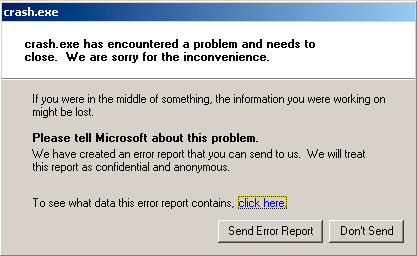
\includegraphics[width=0.6\textwidth]{OS/SEH/1/crash_xp1.png}
\caption{Windows XP}
\end{figure}

\begin{figure}[H]
\centering
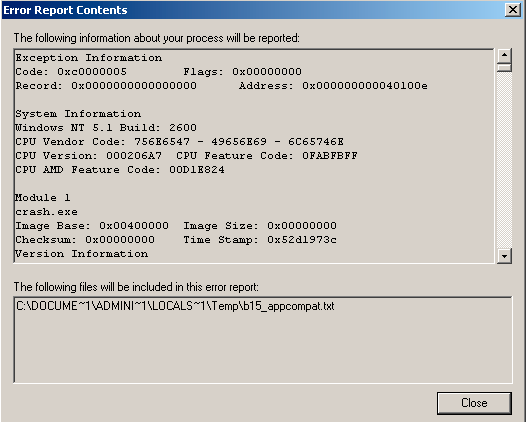
\includegraphics[width=0.6\textwidth]{OS/SEH/1/crash_xp2.png}
\caption{Windows XP}
\end{figure}

\begin{figure}[H]
\centering
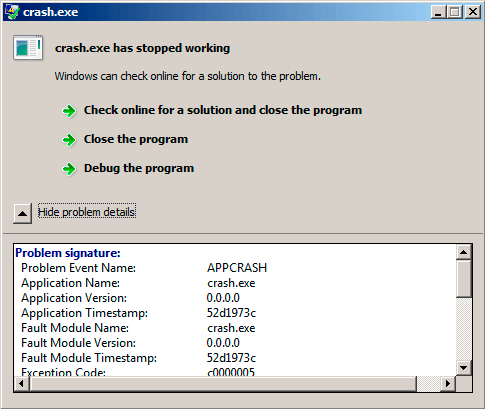
\includegraphics[width=0.6\textwidth]{OS/SEH/1/crash_win7.png}
\caption{Windows 7}
\end{figure}

\begin{figure}[H]
\centering
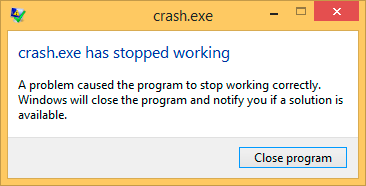
\includegraphics[width=0.6\textwidth]{OS/SEH/1/crash_win81.png}
\caption{Windows 8.1}
\end{figure}

Früher wurde dieser Handler Dr. Watson
genannt.

Einige Entwickler erstellen ihren eigenen Handler, der Informationen über den Absturz
des Programms zu ihnen selbst schickt.
\myindex{Windows!Win32!SetUnhandledExceptionFilter()}
Dieser wird mit der Funktion \TT{SetUnhandledExceptionFilter()} registriert und aufgerufen,
wenn das \ac{OS} keine andere Möglichkeit hat die Ausnahme zu behandeln.
\myindex{\oracle}
Ein Beispiel ist \oracle die eine riesige Menge an möglichen Informationen über die \ac{CPU}
und den Zustand des Speichers sammelt.

Nachfolgend wird ein eigener, einfacher Ausnahme-Handler erstellt.
Dieses Beispiel basiert auf dem Beispiel von \PietrekSEH und muss mit der SAFESEH-Option
kompiliert werden: \TT{cl seh1.cpp /link /safeseh:no}.
Mehr über SAFESEH befindet sich hier: \href{http://msdn.microsoft.com/en-us/library/9a89h429.aspx}{MSDN}.

\lstinputlisting[style=customc]{OS/SEH/1/1.cpp}

Das FS:Segment-Register zeigt unter Win32 auf die \ac{TIB}.

Das erste Element der \ac{TIB} ist ein Zeiger auf den letzten Handler der Kette.
Wir sichern den Stack und speichern hier die Adresse unseres Handlers.
Die Struktur heißt \TT{\_EXCEPTION\_REGISTRATION}. Dabei handelt es sich um eine
einfach-verkette Liste, deren Elemente direkt auf dem Stack gesichert werden.

\begin{lstlisting}[caption=MSVC/VC/crt/src/exsup.inc,style=customasmx86]
_EXCEPTION_REGISTRATION struc
     prev    dd      ?
     handler dd      ?
_EXCEPTION_REGISTRATION ends
\end{lstlisting}

Jedes \q{handler}-Feld zeigt auf einen Handler und jedes \q{prev}-Feld zeigt auf den
vorherigen Eintrag auf dem Stack.
Der letzte Eintrag hat \TT{0xFFFFFFFF} (-1) im \q{prev}-Feld.

\begin{center}
\begin{tikzpicture}[thick,scale=0.75, every node/.style={scale=0.75}]
	\tikzstyle{every path}=[thick]
	\tikzstyle{undefined}=[draw,rectangle,minimum height=1cm, minimum width=3.5cm, text width=3.5cm]
	\tikzstyle{node}=[draw,rectangle,minimum height=1cm, minimum width=3.5cm, text width=3.5cm, fill=gray!20]
	
	\node[node] (fs) [minimum width=1.5cm, text width=1.5cm] {FS:0};

	\node[node] (tib1) [right=1.5cm of fs] {+0: \_\_except\_list};
	\node[undefined] (tib2) [below of=tib1] {+4: \dots};
	\node[undefined] (tib3) [below of=tib2] {+8: \dots};
	\node (tib_text) [above of=tib1] {TIB};
	
	\draw [->] (fs.east) -- (tib1.west);

	\node[undefined] (u1) [text centered, right=2.5cm of tib1] {\dots};
	\node [node] (n1prev) [below of=u1] {Prev=0xFFFFFFFF};
	\node [node] (n1handler) [below of=n1prev] {Handle};
	\node [node] (n1handler_text) [right=1cm of n1handler] {\HandlerFunction};
	\draw [->] (n1handler.east) -- (n1handler_text.west);
	\node[undefined] (u2) [text centered, below of=n1handler] {\dots};
	\node [node] (n2prev) [below of=u2] {Prev};
	\node [node] (n2handler) [below of=n2prev] {Handle};
	\node [node] (n2handler_text) [right=1cm of n2handler] {\HandlerFunction};
	\draw [->] (n2handler.east) -- (n2handler_text.west);
	\node[undefined] (u3) [text centered, below of=n2handler] {\dots};
	\node [node] (n3prev) [below of=u3] {Prev};

	\node [node] (n3handler) [below of=n3prev] {Handle};
	\node [node] (n3handler_text) [right=1cm of n3handler] {\HandlerFunction};
	\draw [->] (n3handler.east) -- (n3handler_text.west);
	\node[undefined] (u4) [text centered, below of=n3handler] {\dots};
	\node (stack_text) [above of=u1] {\RU{Стек}\EN{Stack}};
	
	\node (n2block_pt1) [inner sep=0pt, above left=0cm and 0cm of n2prev] {};
	\node (n2block_pt2) [inner sep=0pt, above left=0cm and 0.5cm of n2prev] {};
	\draw [->] (n3prev.west) .. controls +(left:0.5cm) and (n2block_pt2) .. (n2block_pt1);

	\node (n1block_pt1) [inner sep=0pt, above left=0cm and 0cm of n1prev] {};
	\node (n1block_pt2) [inner sep=0pt, above left=0cm and 0.8cm of n1prev] {};
	\draw [->] (n2prev.west) .. controls +(left:0.8cm) and (n1block_pt2) .. (n1block_pt1);
	
	\node (n3block_pt1) [inner sep=0pt, above left=0cm and 0cm of n3prev] {};
	\node (n3block_pt2) [inner sep=0pt, above left=0cm and 1.25cm of n3prev] {};
	\draw [->] (tib1.east) .. controls +(right:1.25cm) and (n3block_pt2) .. (n3block_pt1);


\end{tikzpicture}
\end{center}


Nachdem unser Handler installiert wurde, wird \TT{RaiseException()}
\footnote{\href{http://msdn.microsoft.com/en-us/library/windows/desktop/ms680552(v=vs.85).aspx}{MSDN}} aufgerufen.
Dies ist eine Benutzer-Ausnahme.
Der Handler überprüft diesen Code.
Ist der Code \TT{0xE1223344}, wird \TT{ExceptionContinueExecution} zurückgegeben,
was bedeutet, dass der CPU-Zustand korrigiert wurde (in der Regel in den EIP-/ESP-Registern)
und anschließend das \ac{OS} die Ausführung fortsetzen kann.
Wenn der Code leicht verändert wird, so gibt der Handler \TT{ExceptionContinueSearch} zurück,
und das \ac{OS} wird andere Handler aufrufen.
Es ist unwahrscheinlich, dass ein Handle gefunden werden kann, weil keine Informationen
(oder Quellcode) darüber vorliegt.
Der Standard-Windows-Dialog wird mit einem Hinweis auf einen Prozess-Absturz aufgerufen.

Was ist der Unterschied zwischen einer System-Ausnahme und einer User-Ausnahme?
Hier sind die Ausnahmen des Systems:

\small
\begin{center}
\begin{tabular}{ | l | l | l | }
\hline
\HeaderColor win in WinBase.h definiert & 
\HeaderColor wie in ntstatus.h definiert & 
\HeaderColor Wert \\
\hline
EXCEPTION\_ACCESS\_VIOLATION          & STATUS\_ACCESS\_VIOLATION           & 0xC0000005 \\
\hline
EXCEPTION\_DATATYPE\_MISALIGNMENT     & STATUS\_DATATYPE\_MISALIGNMENT      & 0x80000002 \\
\hline
EXCEPTION\_BREAKPOINT                & STATUS\_BREAKPOINT                 & 0x80000003 \\
\hline
EXCEPTION\_SINGLE\_STEP               & STATUS\_SINGLE\_STEP                & 0x80000004 \\
\hline
EXCEPTION\_ARRAY\_BOUNDS\_EXCEEDED     & STATUS\_ARRAY\_BOUNDS\_EXCEEDED      & 0xC000008C \\
\hline
EXCEPTION\_FLT\_DENORMAL\_OPERAND      & STATUS\_FLOAT\_DENORMAL\_OPERAND     & 0xC000008D \\
\hline
EXCEPTION\_FLT\_DIVIDE\_BY\_ZERO        & STATUS\_FLOAT\_DIVIDE\_BY\_ZERO       & 0xC000008E \\
\hline
EXCEPTION\_FLT\_INEXACT\_RESULT        & STATUS\_FLOAT\_INEXACT\_RESULT       & 0xC000008F \\
\hline
EXCEPTION\_FLT\_INVALID\_OPERATION     & STATUS\_FLOAT\_INVALID\_OPERATION    & 0xC0000090 \\
\hline
EXCEPTION\_FLT\_OVERFLOW              & STATUS\_FLOAT\_OVERFLOW             & 0xC0000091 \\
\hline
EXCEPTION\_FLT\_STACK\_CHECK           & STATUS\_FLOAT\_STACK\_CHECK          & 0xC0000092 \\
\hline
EXCEPTION\_FLT\_UNDERFLOW             & STATUS\_FLOAT\_UNDERFLOW            & 0xC0000093 \\
\hline
EXCEPTION\_INT\_DIVIDE\_BY\_ZERO        & STATUS\_INTEGER\_DIVIDE\_BY\_ZERO     & 0xC0000094 \\
\hline
EXCEPTION\_INT\_OVERFLOW              & STATUS\_INTEGER\_OVERFLOW           & 0xC0000095 \\
\hline
EXCEPTION\_PRIV\_INSTRUCTION          & STATUS\_PRIVILEGED\_INSTRUCTION     & 0xC0000096 \\
\hline
EXCEPTION\_IN\_PAGE\_ERROR             & STATUS\_IN\_PAGE\_ERROR              & 0xC0000006 \\
\hline
EXCEPTION\_ILLEGAL\_INSTRUCTION       & STATUS\_ILLEGAL\_INSTRUCTION        & 0xC000001D \\
\hline
EXCEPTION\_NONCONTINUABLE\_EXCEPTION  & STATUS\_NONCONTINUABLE\_EXCEPTION   & 0xC0000025 \\
\hline
EXCEPTION\_STACK\_OVERFLOW            & STATUS\_STACK\_OVERFLOW             & 0xC00000FD \\
\hline
EXCEPTION\_INVALID\_DISPOSITION       & STATUS\_INVALID\_DISPOSITION        & 0xC0000026 \\
\hline
EXCEPTION\_GUARD\_PAGE                & STATUS\_GUARD\_PAGE\_VIOLATION       & 0x80000001 \\
\hline
EXCEPTION\_INVALID\_HANDLE            & STATUS\_INVALID\_HANDLE             & 0xC0000008 \\
\hline
EXCEPTION\_POSSIBLE\_DEADLOCK         & STATUS\_POSSIBLE\_DEADLOCK          & 0xC0000194 \\
\hline
CONTROL\_C\_EXIT                      & STATUS\_CONTROL\_C\_EXIT             & 0xC000013A \\
\hline
\end{tabular}
\end{center}
\normalsize

Nachfolgend wie der Code aufgebaut ist:

\begin{center}
\begin{bytefield}[bitwidth=0.03\linewidth]{32}
\bitheader[endianness=big]{31,29,28,27,16,15,0} \\
\bitbox{2}{S} & 
\bitbox{1}{U} &
\bitbox{1}{0} & 
\bitbox{12}{Facility code} &
\bitbox{16}{Fehler-Code}
\end{bytefield}
\end{center}

S ist ein einfacher Status-Code:
11---Fehler;
10---Warnung;
01---Information;
00---Erfolgreich.
U---Kennzeichnet ob es sich um User-Code handelt.

Dies erklärt, warum wir oben den Wert 0xE1223344 gewählt haben---E\textsubscript{16}
(1110\textsubscript{2}) 0xE (1110b) 
bedeutet, dass es sich um eine User-Ausnahme handelt; 2) ein Fehler vorliegt.

Genaugenomen funktioniert dieses Beispiel jedoch auch gut ohne diese höherwertigen Bits.

Anschließend versuchen wir einen Wert von der Speicheradresse 0 zu lesen.

Natürlich befindet sich hier nichts unter Win32, womit eine Ausnahme geworfen wird.

Der allererste Handler wird aufgerufen (der von oben) und prüft ob der Code der Konstante\\
\TT{EXCEPTION\_ACCESS\_VIOLATION} entspricht.

Der Code der von der Adresse an der Speicherstelle 0 liest, sieht wie folgt aus:

\lstinputlisting[style=customasmx86,caption=MSVC 2010]{OS/SEH/1/1_fragment.asm}

Ist es möglich diese Fehler \q{on the fly} zu beheben und mit der Programmausführung
fortzufahren?

In der Tat ist dies möglich, da unser Ausnahme-Handler den \EAX-Wert beheben und das
\ac{OS} diese Anweisung ein weiteres Mal ausführen kann.
Das ist was wir tun. \printf gibt 1234 aus, weil \EAX nach der Ausnahmebehandlung nicht
mehr 0 ist sondern die Adresse der globalen Variable \TT{new\_value} enthält.
Die Ausführung wird fortgesetzt.

Das ist was passiert: die Speicherverwaltung in der \ac{CPU} signalisiert einen Fehler und
die \ac{CPU} stoppt den Thread, findet die passende Ausnahmebehandlung im Windows-Kernel
welche wiederum nacheinander alle Handler in der \ac{SEH}-Kette aufruft.

Hier wird MSVC 2010 genutzt, aber es gibt natürlich keine Garantie, dass \EAX für diesen
Zeiger genutzt wird.

Dieser Adresse-Ersatz-Trick dient der Veranschaulichung der internen Vorgänge von \ac{SEH}.
Dennoch ist es schwierig einen realen Einsatz für das Fixen eines Fehlers \q{on-the-fly}
zu finden.

Warum sind die SEH-Einträge direkt auf dem Stack gespeichert und nicht irgendwo anders?

Vermutlich ist der Grund, weil das \ac{OS} sich dann nicht um das freigeben der Informationen
kümmern muss. Diese Einträge werden nach dem Ende der Funktion automatisch gesäubert.
\myindex{\CStandardLibrary!alloca()}
Dies entspricht in gewisser Weise alloca(): (\myref{alloca}).
